%% ----------------------------------------------- %%
%%            Graphical user interface             %%
%% (documentation chapter for the FilmTit project) %%
%% ----------------------------------------------- %%

The Graphical User Interface (GUI) is the part of the application that is loaded by the user in his web browser. It is written mostly in Java but compiled by the Google Web Toolkit (GWT) into JavaScript. Its main tasks are

\begin{itemize}
\item visualisation of the application and communication with the user in a user-friendly way, especially providing an efficient translation workspace adapted for translation of movie subtitles
\item communication with the User Space (see Chapter~\ref{chap:userspace}) through the Remote Procedure Calls (see Chapter~\ref{chap:communication}), especially to provide the user with translation suggestions from the core translation memory (see Chapter~\ref{chap:core}) and for data persistence
\end{itemize}

\section{Goals}
% (Honza)
Our main goal is to offer a tool for the translators of the movie subtitles as easy and effective to use as possible. With the capabilities of the current web browsers, we decided to make FilmTit a web-based application, therefore sparing the user the need to download and install anything.

\section{Google Web Toolkit}
% (Honza and Ruda)
The web-based user interface representing the client part of the FilmTit application is based on the Google Web Toolkit (GWT) framework. This technology is a development toolkit for building and optimizing browser-based applications %\citep{Gwtweb}
and is based on the idea of compilation of Java source code into JavaScript. Therefore, it enables us to write in Java even on the client side, but preserving most of the advantages of web application accessibility for the user.

The official description of GWT is as follows:

Google Web Toolkit (GWT) is a development toolkit for building and optimizing complex browser-based applications. Its goal is to enable productive development of high-performance web applications without the developer having to be an expert in browser quirks, XMLHttpRequest, and JavaScript. GWT is used by many products at Google, including Google Wave and the new version of AdWords. It's open source, completely free, and used by thousands of developers around the world.


%More about decision for using GWT can be found in \ref{subsubsec:implementation:gwt}.
\subsection{Reasons for Using GWT and Discussion}
\label{sec:reasonsForGWT}

We decided to use GWT for several reasons.
One reason is that it integrates very well with the rest of the 
application, which is written in Java. A prominent example is the 
communication between GUI and User Space. Not only is the interface 
defined by one simple Java class ({\tt FilmTitService}), which is then 
used both by the GUI and the User Space, but thanks to GWT we are even 
able to use exactly the same classes (placed in {\tt cz.filmtit.share}) 
in GUI and in User Space and send them easily through the {\tt 
FilmTitService} interface. Thus, we avoided the trouble of having to keep 
each of these classes in two versions, Java and JavaScript, together with 
mappings to and from the transport format. (In fact, all of these do 
exist in the application, but only in the compiled code, completely 
hidden from the developer.)

However, there is a downside, which could have been expected but is 
difficult to manage properly. It is obvious that GWT does not support 
everything that exists in Java -- instead, it supports only a subset of 
Java, with many GWT-specific additions. This is perfectly reasonable, 
and, as the subset supported is large enough, should not cause any 
problems. The IDE does not provide much support in this area, so often the only thing 
that a developer can rely on are Internet forums. Luckily, GWT is used by 
many developers and most of the issues that we encountered had already 
been solved by others (although sometimes the only solution was not a 
nice or clean one, such as having to implement some methods directly in 
JavaScript). Still, we spent much debugging time on problems that were actually problems of GWT that had to be worked around, instead of being problems of our code.

A requirement that we had for the web technology was to offer an IDE (in GWT realized by a plugin for Eclipse IDE, similarly applicable also for the IntelliJ IDE), possibly with debugging support. In GWT, there is a dedicated Development Mode for these debugging purposes, sparing the developer the need of recompiling all the GWT code for testing after each change. This proved to be very efficient in the first phases of the development when the GUI module was developed independently and, although it turned out to be quite difficult to set up the Development Mode once the GUI module was integrated with the rest of the project, it remained one of the most useful features of GWT.

Another option that we found useful is the possibility to directly insert real Javascript code into GWT methods. Although it is not very clean and cannot benefit from some of the features of GWT, it is sometimes the only way to do something that is supported in Javascript but unsupported in GWT.

An important point also was that GWT is freeware, or more precisely, is licensed under the Apache License, v.~2.0, with several third-party software libraries included in its distribution under other freeware licenses. It is even open-source, from which we benefited occasionally when examining the source code to understand some of its unexpected behavior, or even to extend some of its classes, overriding their behavior to suit our needs.

Although GWT can be integrated into a Maven project, it was far from flawless and a significant amount of time had to be spent on making everything work together, including maintaining the IDE support. We managed to do that in the end, but we had expected this to be much easier. 
The main reason (but not the only one) is the specific directory structure, different for the Maven project and for the GWT project, which has to be adjusted in the configuration of both the Maven plugins and the IDE.
And still after setting everything correctly, some features remained unavailable to some of us, e.g.\ running GUI in Development Mode using Eclipse IDE.

To conclude, we are happy that we decided to use GWT because of the benefits it brought to us, but we were disappointed by the number of complications that it brought as well. Were we to decide on a web framework to use for a similar project, we would still have to consider our decision carefully.


\subsection{Browser Support and Optimization}
GWT also provides a feature which makes the final web application similar in different major browsers and optimized to a certain degree for each of them. This feature is called {\em deferred binding} and it is based on generating different versions of the JavaScript code during compile time, only one of which needs to be loaded by a particular client browser at runtime. This process is by default maintained by the GWT compiler itself, so that the developer does not have to worry about it.

However, this ``unification'' is not complete, nor it is intended to be. It covers only the bigger and more crucial differences of the code behavior among various browsers, but does not address some slight variancies e.g.\ in design of the basic elements (and their most common behavior). This seems reasonable, because forcing each browser to interpret the code in the exact same way would mean hardcoding almost everything from scratch and not using many of their provided features, which would be probably impossible anyway. Nevertheless, some of these ``slight differences'' which we have encountered proved to be quite crucial for our intended design (especially in the event-handling domain), so lots of work had to be done to reasonably unify the application's behavior even among the major browsers.

Still, our hope is that GWT development will continue and will keep up with the development of web browsers, allowing us to provide browser-up-to-date versions of FilmTit simply by acquiring a new version of GWT and recompiling the project. Currently, the application works well with Opera v.~12
Firefox v.~14, Chrome v.~21 and Safari v.~5.1.5 or higher.


\subsection{Designing by UiBinder}
Another very useful and comfortable feature of the GWT for designing the user interface is the UiBinder. The idea behind this approach is to design the visual structure of the page (or its part) in an HTML-like way (this is called the {\em UiBinder template}) and its behavior and functionality in a Java class (called the {\em owner class} for the template). The UiBinder itself is then an object binding these two approaches together. This style of creating the web application supports the respected best practice to divide the visual design and the functionality. It also allows to create the web page's appearance in a way which is more natural to web designers (e.g. HTML-like), as well as more readable and modifiable. Other advantages include supposedly better performance (as the browsers can better optimize the rendering from the UiBinder templates than from the heavier-weight Java-based widgets and panels) and support for internationalization (not used by FilmTit at the moment).

The actual source code of a page designed this way (or of its segment) then consists of a file with the *.ui.xml Ui-Binder template (where also the style definition can be included directly) and a corresponding *.java owner class, where the elements of the template can be accessed as widgets (as well as made accessible to other classes). The owner class then can be simply instantiated and plugged into an existing design just like any other widget.

\subsection{Twitter Bootstrap Library}
For enhancing the visual appearance of our application to a modern look without a professional graphic designer, we have decided to use an existing open-source library for GWT which displays the page elements (and their groups) in the style of the Twitter pages. This library is called GWT-Bootstrap and is easily applicable with the UiBinder-style designing. It is also still a live project, so there is a hope that more features would be available in the possible future development.

Similarly to other third-party libraries used by FilmTit, the GWT-Bootstrap library is attached as a Maven dependency and downloaded automatically from its own Maven repository.



\section{GUI Structure}
% (Honza/Ruda)

The GUI is contained in the package {\tt cz.filmtit.client} (not {\tt cz.filmtit.gui} for ``historical'' reasons -- ``client'' is the default package name in GWT for the client side of a web application). All of it is written in Java (in its subset that is GWT-compilable to JavaScript), with occasional methods with bodies written directly in JavaScript (for reasons clarified in \ref{subsubsec:implementation:gwt}). Thus, the GUI can actually only be compiled to Javascript.

The GUI also makes use of the shared classes (package {\tt cz.filmtit.share}, see~\ref{sec:shared_classes}), which are written using only the intersection between standard Java and GWT-compilable Java and are therefore fully compilable both to Javascript and to Java bytecode.

Some settings have to be done via several resource files in the webapp directory. (This is required by the Java Servlets technology used to deploy the application.)

\subsection{Gui.java}

The main class is Gui.java. It defines the web application itself, providing an entry point, initialization methods, logging methods and access to page switching. It also contains fields that are considered global, such as the {\tt sessionID} of the currently logged in user.
It behaves as a static class, except for the {\tt onModuleLoad()} method required by GWT, which corresponds to the {\tt main()} function.

\subsection{Pages}

\subsubsection{GWT -- discussion}
\label{gui:gwt}
Very soon, we found out a week point of GWT: it has nearly no native support for multiple pages. This was quite a surprising issue to us, since in any other web development technology or framework that we know, creating a new page and switching pages are really simple tasks. GWT, however, uses the idea of having one HTML file and one JavaScript file only that handle everything. (It is technically possible to create multiple pages by creating multiple GWT projects, each corresponding to one page, but this is not recommended for many good reasons.)

The GWT way of switching pages is by replacing the contents of the Root Panel (which represents the visible part of a page), or any other Panel placed within the Root Panel (which we decided to use so that some elements, such as the menu, are present on all pages). The switching is done without reloading, simply by creating an instance of the new page and directly setting it as the contents of the panel (without any convenience functions for that to our knowledge).

All the pages have the same URL by default, but GWT offers the History class for changing the URL and reacting to changes to URL (however, it is not linked to page switching by design -- this remains for each programmer to do by himself). There are also {\tt Hyperlink} widgets, which represent a link to a different page, with the default action being changing the URL and invoking the appropriate handler (a {\tt ValueChangeHandler}).
The URL contains an anchor with the name of the page (e.g.\ {\tt \#DocumentCreator} or {\tt \#WelcomeScreen}), and the History class is able to provide the name of the anchor to the user and to invoke the ValueChangeHandler when the URL changes.

We decided to use the {\tt History} class and {\tt Hyperlinks} to implement the menu and page switching. We create a {\tt PageHandler} class which implements the {\tt ValueChangeHandler} -- it turns the anchor string into a value of Page enum, checks whether the requested page can be loaded (especially based on the user log in / log out state) and loads the appropriate page. It also provides public methods to other parts of GUI so that they can switch pages, modifying the URL at the same time (so that the browser refresh works as expected).

However, we encountered one issue with the {\tt Hyperlinks}: the {\tt ValueChangeHandler} is invoked only if the value of URL changes, which means that if the user clicks a menu link which points to the page loaded (e.g. while creating a document, the user decides to restart and clicks the document creator link), the handler is not invoked. As this behavior is hard-coded into the {\tt Hyperlink} class, we had to abandon the Hyperlinks and used {\tt NavLinks} instead (a simple link with no default interaction with the History), with click handlers invoking the {\tt ValueChangeHandler}.

We also had a discussion about the expected page to be loaded in various situations. E.g.\ if the user is in Translation Workspace and logs out, the URL page parameter stayed on Translation Workspace by default, although Welcome Screen is displayed instead because a logged out user does not have access to Translation Workspace. If he then logged back in without switching the page, the document he had opened before logging out was reopened again.

Eventually, the behavior was modified so that the URL is always changed to Welcome Page when the users explicitly log out, but the URL is not modified if the users are logged out automatically, typically because their Session ID expire. Reasoning: if they were logged out implicitly, it is probable that they did not want that and would like to continue with their work as soon as possible. However, if they logged out explicitly, they probably finished their work and expects the application to be ``closed'', i.e.\ not remembering the last state of their work.


\subsubsection{Structure}

The subpackage {\tt cz.filmtit.client.pages} defines the pages of the application.
Please refer to the sitemap figure \ref{fig:sitemap} for an overview of the pages, which are:

\begin{itemize}
\item {\tt DocumentCreator}, used to create a new document
\item {\tt TranslationWorkspace}, the main page of the application where the actual translations take place
\item {\tt UserPage}, providing listing of user documents and the possibility to edit them
\item {\tt Settings}, enabling the user to change several settings, such as his password or the maximum number of translation suggestions to show
\item {\tt WelcomeScreen}, displayed as the first page of the application
\item {\tt Help}, showing the user manual of the application
\item {\tt PlayerInfo}, showing guidelines on how to run the media player
\item {\tt PlayerDemo}, showing a sample video for the user to test the media player
\item {\tt ChangePassword}, used as the target of the password change link sent by e-mail to users who forget their password, enabling them to set a new password
\item {\tt AuthenticationValidationWindow}, a special page that receives OpenID authentication data from an OpenID provider and passes them to User Space for validation
\item {\tt Blank}, a special page with no contents and is used to temporarily hide the contents of another page
\end{itemize}

\begin{figure}
\begin{center}
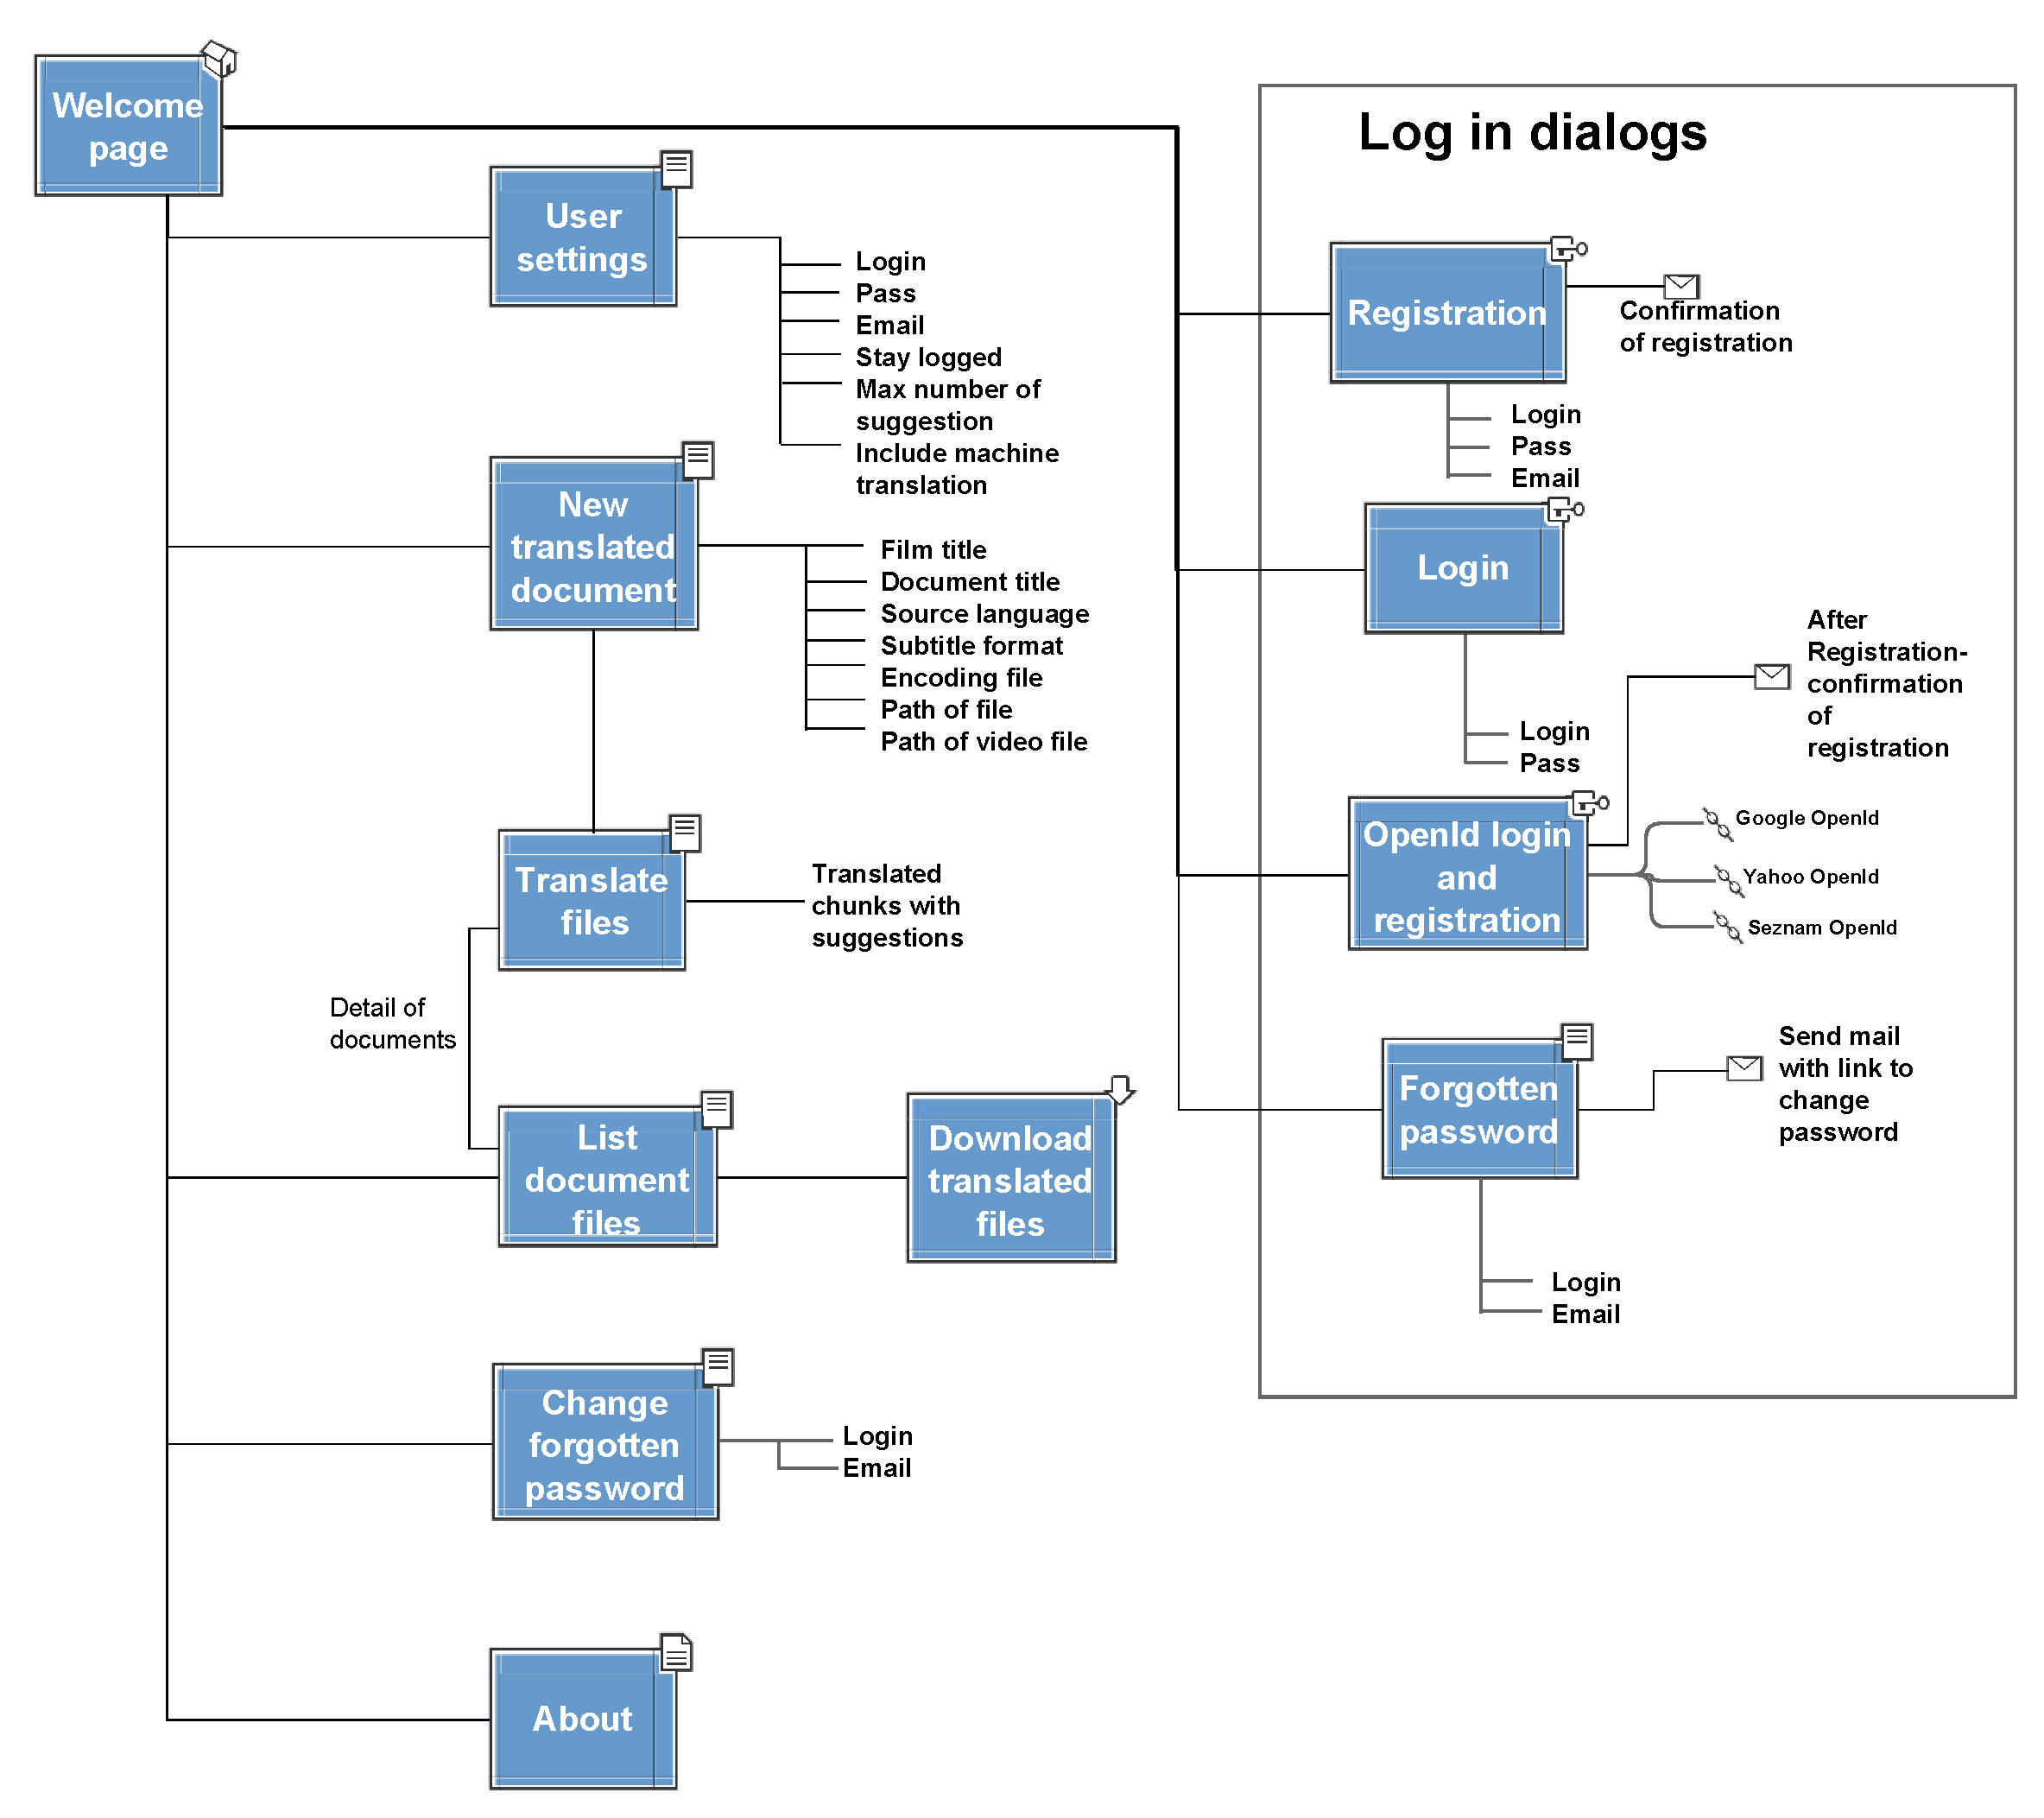
\includegraphics[scale=0.4]{figures/sitemap.pdf}
\end{center}
\caption{Site map of the application}
\label{fig:sitemap}
\end{figure}

As was already mentioned, each page has its layout and function separated as much as possible, with the function being defined in a <page>.java file and the layout in a UiBinder <page>.ui.xml file.

The pages package also contains the {\tt GuiStructure}, which defines the content panel, into which the individual pages are loaded, and the top menu, which enables the users to log in and out and to switch pages.

A page is created and loaded by calling its constructor, which may require some parameters (such as {\tt documentID} for {\tt TranslationWorkspace}).
Page loading and switching is handled by the {\tt PageHandler}, which also provides support for URLs: e.g.\ the About page can be accessed by a URL {\tt http://server/\#About} or {\tt http://server/?page=About} (the first one being the default), with the help of the GWT History class.

\subsection{Dialogs}

Apart from pages, the GUI also contains several dialogs that can be displayed on top of a page. The dialogs are defined in the {\tt cz.filmtit.client.dialogs} subpackage and are typically extended from the abstract {\tt Dialog} class in the same package.

The {\tt Dialog} class defines a modal dialog container and an ``interface'' to be used to handle the dialogs -- all dialogs should only be accessed via this interface (except for their creation, which is invoked by their constructor).
The interface methods are especially
{\tt deactivate()}, {\tt reactivate()}, {\tt showInfoMessage()}, {\tt showErrorMessage()} and {\tt close()}. To deactivate a dialog means to disable all of its active elements so that the user cannot interact with it and must wait for the dialog being reactivated or closed.

The Dialogs defined by the application are:
\begin{itemize}
\item {\tt LoginDialog}, used for logging in and related functions,
\item {\tt SessionIDPollingDialog}, used when waiting for OpenID login process to complete,
\item {\tt MediaSelector}, used to select the correct movie or series of a newly created document or when changing the document's movie title,
\item {\tt TimeEditDialog}, used to edit timing of subtitle items,
\item {\tt DownloadDialog}, which enables the user to download the translated subtitle file,
\item {\tt GoingOfflineDialog}, offering the user to turn on the Offline Mode, and
\item {\tt GoingOnlineDialog}, offering the user to upload data from Offline Mode when the user goes back online
\end{itemize}

\subsection{Remote Procedure Calls Implementation}

Each RPC is in GUI represented by a class from the {\tt cz.filmtit.client.callables} subpackage. The name of the class is typically similar to the RPC name -- e.g.\ for {\tt deleteDocument} RPC it is the {\tt DeleteDocument }class. Each of these classes is extended from the {\tt Callable superclass}, which will be described in the next section.

The RPC is invoked by creating a new instance of the callable class, providing the neccessary parameters in the constructor -- e.g. to invoke the {\tt simpleLogin()} RPC with the username and password parameters, one simply calls {\tt new SimpleLogin(username, password)}. A reference to the instance usually does not have to be kept, since the actions to take on success or failure of the RPC are already hard-coded into the onSuccessAfterLog and onFailureAfterLog methods of the class.

\subsubsection{Callable}

The institute of the {\tt Callable} superclass of all RPC classes has several purposes:

\begin{itemize}
\item to alleviate the burden of boiler-plate RPC invocation code by providing a wrapper for the ``raw'' RPC call
\item to provide utility methods and default actions, such as error handling
\item to provide actions to be always taken, such as logging of the calls with their parameters, and their results
\item to provide a common structure for all RPCs
\end{itemize}

The Callable class itself implements the {\tt AsyncCallback} interface, implementing the required {\tt onSuccess} and {\tt onFailure} methods; therefore, and instance of its subclass can be directly passed to the asynchronous call as the callback.

The subclasses representing the individual calls must only override the {\tt call()} method, which specifies the actual RPC to be invoked.
They can also modify the default behavior defined by the superclass by overriding several other methods, such as {\tt onSuccessAfterLog}, {\tt onEachReturn}, {\tt onFailureAfterLog}, {\tt onProbablyOffline} etc. This way, the behavior needed can be always achieved, but the default implementation is often sufficient, so the subclasses often override only one or two methods, keeping their code as simple as possible. (The method most often overridden is the {\tt onSuccessAfterLog} method; its default implementation is to do nothing, which is only good for RPCs that do not require any reaction of GUI on their successful return, such as {\tt changeDocumentTitle} or {\tt stopTranslationResults}.)

\subsubsection{Error handling}

If the request fails for any reason, it is retried by default; four attempts are made for each request, always retrying after a short time interval.
Resending the request is the default behavior which the subclasses override in cases where it is obvious that resending will not help (e.g. incorrect e-mail address format or an already existing username on registration).

In case of network problems, both temporary and permanent (this cannot be easily distinguished), the GUI usually receives a {\tt StatusCodeException} with the status code 0. In such case the request is always resent three times before passing control to the {\tt onProbablyOffline} method (this behavior cannot be overridden).

There is also a timeout for each request after which the request is regarded as lost and is retried.

The default action in case of an error is to show the error message in a JavaScript alert window, except for the {\tt InvalidSessionIdException} where the default action is to ask the user to log in again.
The subclasses often override this by showing the message in a Dialog (invoking the {\tt reactivateWithErrorMessage} method of the {\tt Dialog} class), or by ignoring the error completely (e.g.\ when deleting a document, a failure with an {\tt InvalidDocumentIdException}, meaning that the document does not exist, is an error, but there is no need to inform the user because the result is the same as if the RPC succeeded: the document does not exist now.)

Most of the RPCs contain the {\tt sessionID} as one of their parameters to authenticate the user. All of such RPCs can thus throw an {\tt InvalidSessionIdException}, to which the default action is to show the Login Dialog to the user.

\subsection{Offline Mode}
\label{gui:offlinemode}

The Offline Mode offers the users the possibility to continue translating a document even without a connection to the server. Their translations are stored locally in his browser and sent to User Space once they go back online.
Support for storing the data is ensured by the HTML5 Local Storage feature, which provides an in-browser data storage, accessible from JavaScript.
Each object is stored as a pair of a unique string key and a string value (therefore, serialization to string is necessary to store complex objects).



\subsubsection{Motivation}

We decided that the only part that has to be able to work offline is the Translation Workspace, as doing the translation itself is the most time-consuming part of the whole process for a user. We believe that the user can prepare everything while online, wait until the translation suggestions are loaded, and then spend some time offline translating the document.

We also decided to require for the application to stay open while the user goes offline, as it would be difficult to reload the application offline
-- e.g.\ the whole application would have to be stored offline, which we wanted to avoid in the first place by designing FilmTit as a web application.
However, it is obvious that the data created by the user in Offline Mode must be stored locally even if the application is closed.
Thus, only storing {\tt setUserTranslation} calls and invoking them once the user goes back online turned out to be sufficient.


We decided to use HTML5 Local Storage, which is similar to the well-known cookies mechanism from which it evolved.
Like Cookies, the stored object has two ``useful'' string fields, the name (or ``key'') and the contents (or ``value'').
However, the Local Storage has several advantages over cookies:

\begin{itemize}
\item The objects are not sent to the browser on loading the page but are stored and retrieved on request. This would actually be a disadvantage if we wanted to interact with the storage from the server side; however, in our case, being only able to handle the objects from within JavaScript is an advantage.
\item The size limit both for individual objects and for the total amount of data stored is larger.
\item Instead of setting expiry time, the programmer simply decides whether the objects should be stored temporarily (for a browser session) or permanently (which is our case).
\item The API is cleaner.
\end{itemize}

Still, thanks to the similarity of Local Storage to cookies, it would be quite easy to implement a fallback for browsers without Local Storage support using cookies. We decided not to do that because, as far as we know, most browsers installed on users' computers nowadays should support Local Storage. However, we might add this feature in future if there is a need for it.

\subsubsection{Implementation}
The Offline Mode support is separated into three parts: the {\tt LocalStorageHandler}, the {\tt Storable} interface, and classes implementing the interface (i.e. the {\tt SetUserTranslation} class).


\subsubsection{Storable interface}
\label{gui:subsubsec:storable}

This interface defines methods that need to be implemented by a class to be storable in the Local Storage, especially:

\begin{itemize}
\item {\tt toKeyValuePair()} -- to serialize the object into a pair of a key and a value

\item {\tt static fromKeyValuePair(KeyValuePair)} -- a factory method that deserializes the object from a pair of a key and a value (not actually defined by the interface; for a discussion on that matter see Section~\ref{ip:subsubsec:offline})

\item {\tt onLoadFromLocalStorage()} -- invoked by the {\tt LocalStorageHandler} when the user decides to upload the object
\end{itemize}

Each implementing class defines its serialization such that its key uniquely identifies the object and the value contains all data (except for those already contained in the key) needed to reconstruct the object.
(The key and the value are expected to consist of semicolon separated fields by default, but each class can define its own serialization, there are no restrictions other than defined by the String class.)

To store in the Local Storage, the key is extended to a ``full key'' by adding the {\tt classID} (e.g.\ ``SetUserTranslation'') and the {\tt userID} (a long),
so the resulting format of key is:

\begin{center}
full key = {\tt userID@classID:key}
\end{center}
When loading the object from the Local Storage, these added fields are used to indetify the owner of the object and the class to deserialize the object into, and are stripped before passing the key to the {\tt fromKeyValuePair()} method; thus, the class gets the key for deserialization in exactly the same format as it was produced by the class on serialization.

Unlike the key, the value is defined solely by the implementing class and is stored and loaded ``as is''.

The {\tt Storable} interface is currently only implemented by the {\tt SetUserTranslation} class.


\subsubsection{SetUserTranslation}

The {\tt SetUserTranslation} class defines its serialization key and value as follows:

\begin{itemize}
\item key = {\tt documentId;chunkId;partNumber}
\item value = {\tt chosenTranslationPair;userTranslation}
\end{itemize}

The onLoadFromLocalStorage() method implementation invokes the setUserTranslation RPC.

\subsubsection{LocalStorageHandler}

The static {\tt LocalStorageHandler} handles storing and loading of Storable objects to and from the Local Storage.

An important field is a boolean ``online'', which determines whether user is in Online Mode or Offline Mode. Setting this value is eqivalent to switching the Offline Mode on or off.

The {\tt LocalStorageHandler} implements especially the following (static) methods:

\begin{itemize}
\item {\tt storeInLocalStorage} (Storable) -- takes a Storable object, serializes it and stores it into the Local Storage

\item {\tt loadUserObjectsFromLocalStorage()} -- examines the Local Storage and returns a list of objects that belong to the current user

\item {\tt uploadUserObjects()} -- deserializes the loaded objects and invokes their onLoadFromLocalStorage() methods
\end{itemize}

\subsubsection{The Offline Mode operation}

Please see the sequence diagram \ref{gui:sd:offline_mode_1} for the first phase, where the user goes offline and continues working on the translation, and the sequence diagram \ref{gui:sd:offline_mode_2} for the second phase, where the user goes online again and the locally stored data are uploaded to the server.
(For simplicity the diagrams do not show some implementation details;
also, parameters are listed only if they are necessary for understanding the process.)

\begin{figure}[h]
\begin{center}
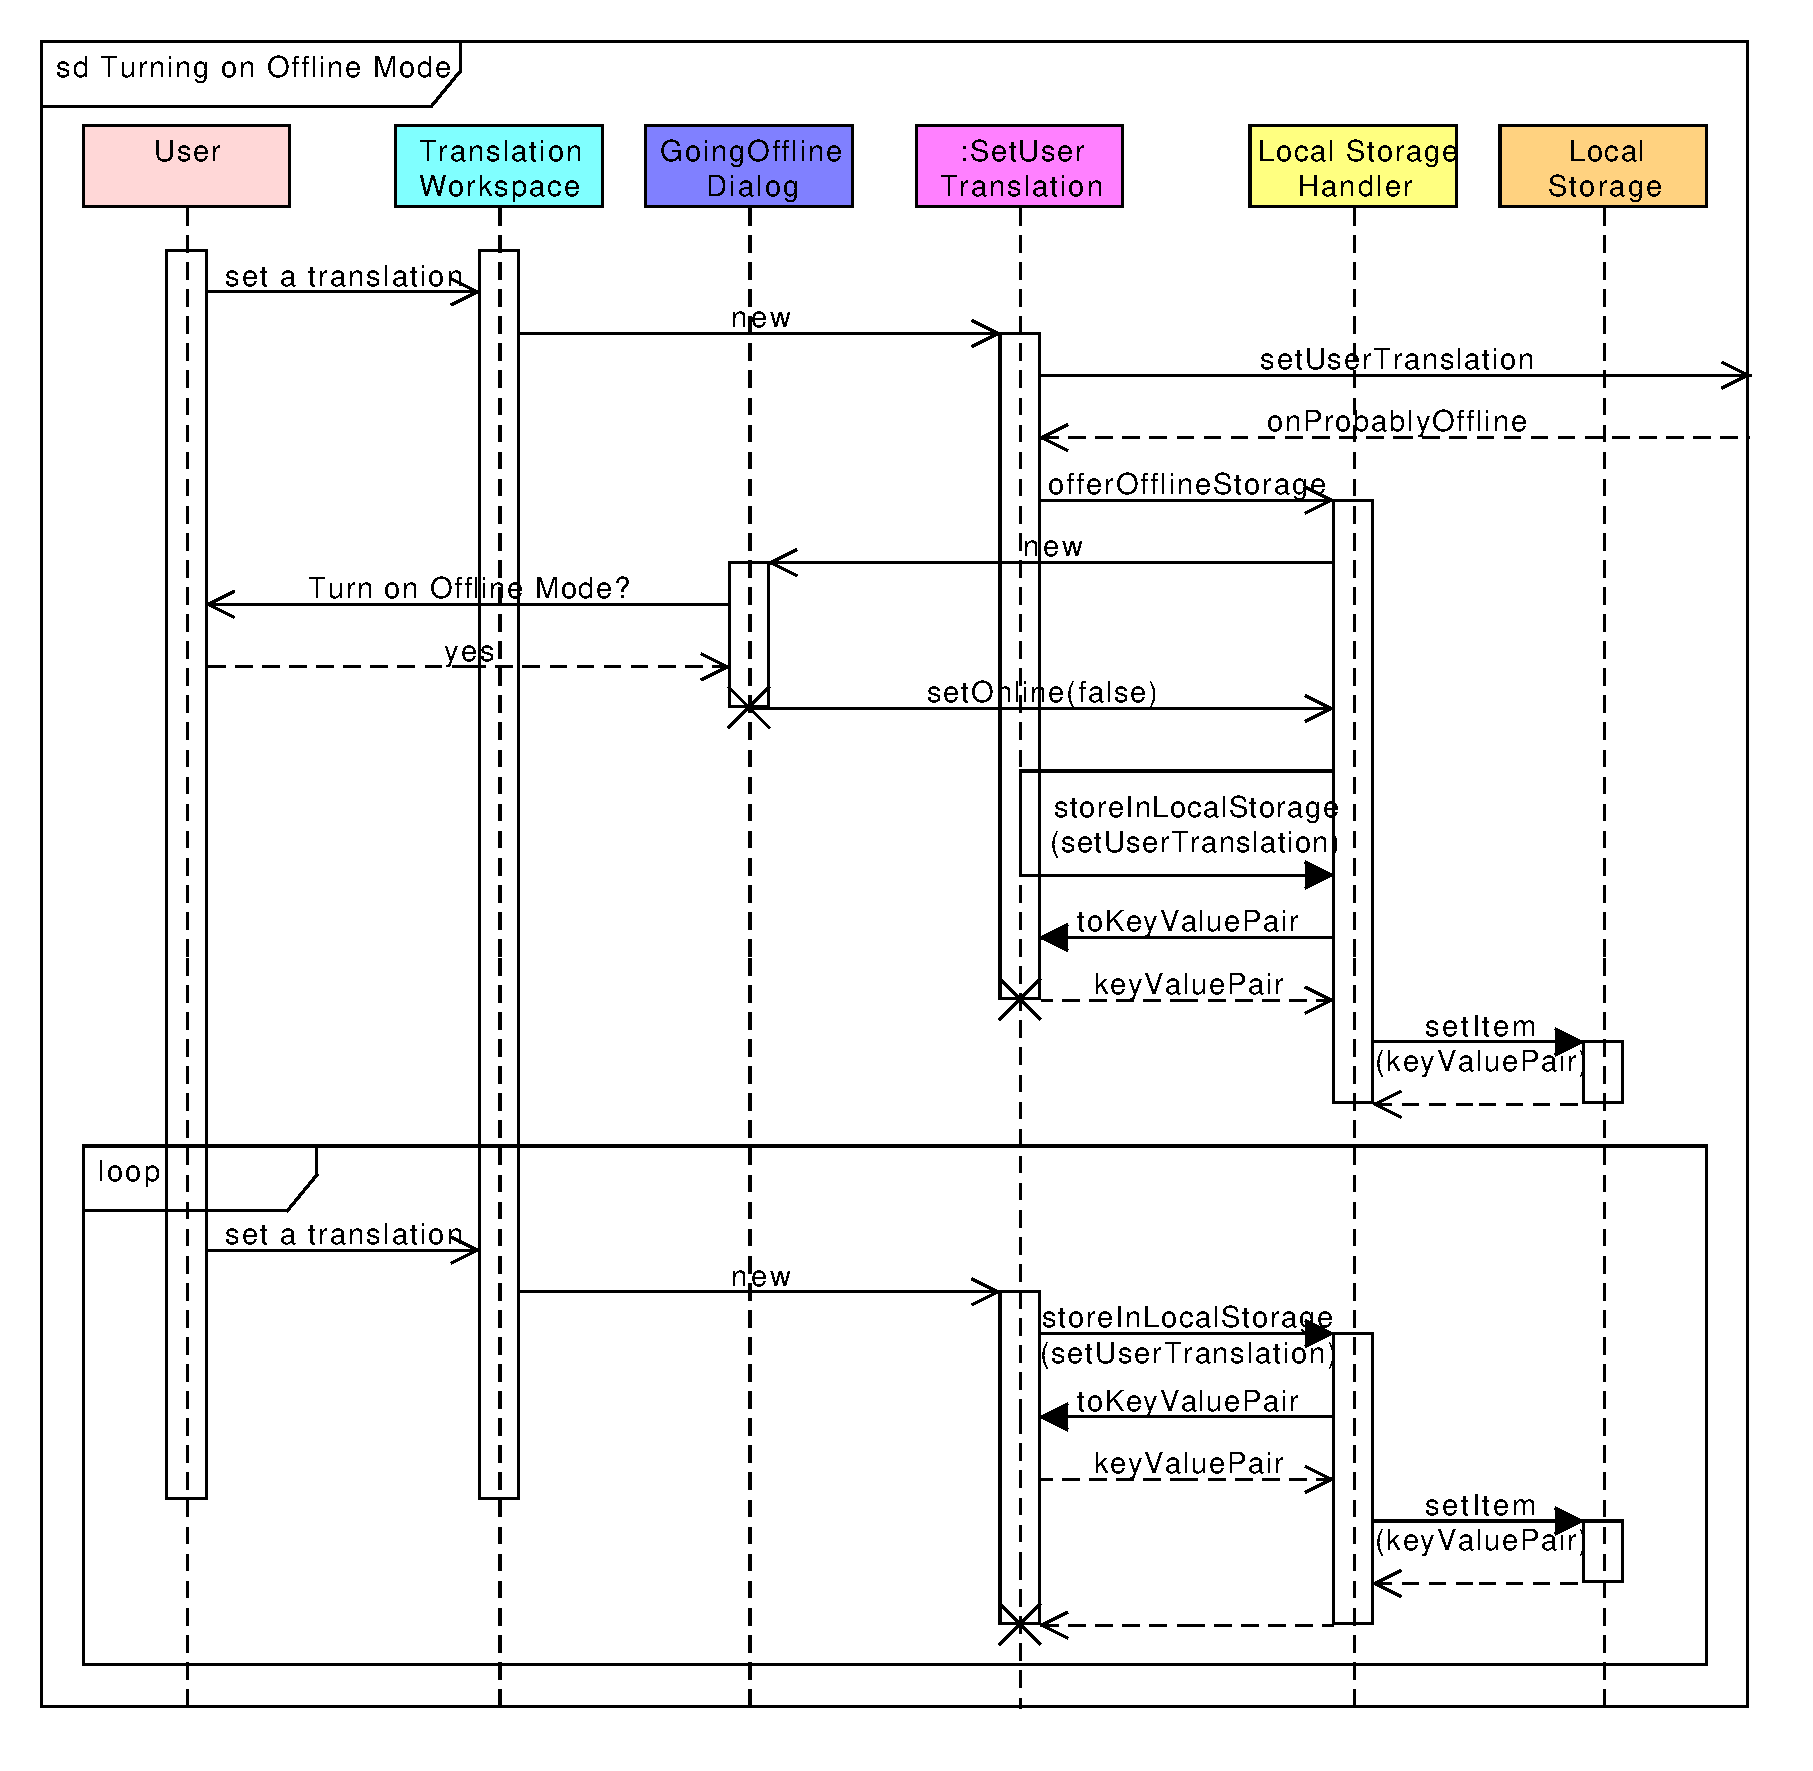
\includegraphics[scale=0.55]{figures/offline_mode_1.pdf}
\end{center}
\caption{Sequence diagram of turning on the Offline Mode and translating the document in Offline Mode.}\label{gui:sd:offline_mode_1}
\end{figure}

\begin{figure}[h]
\begin{center}
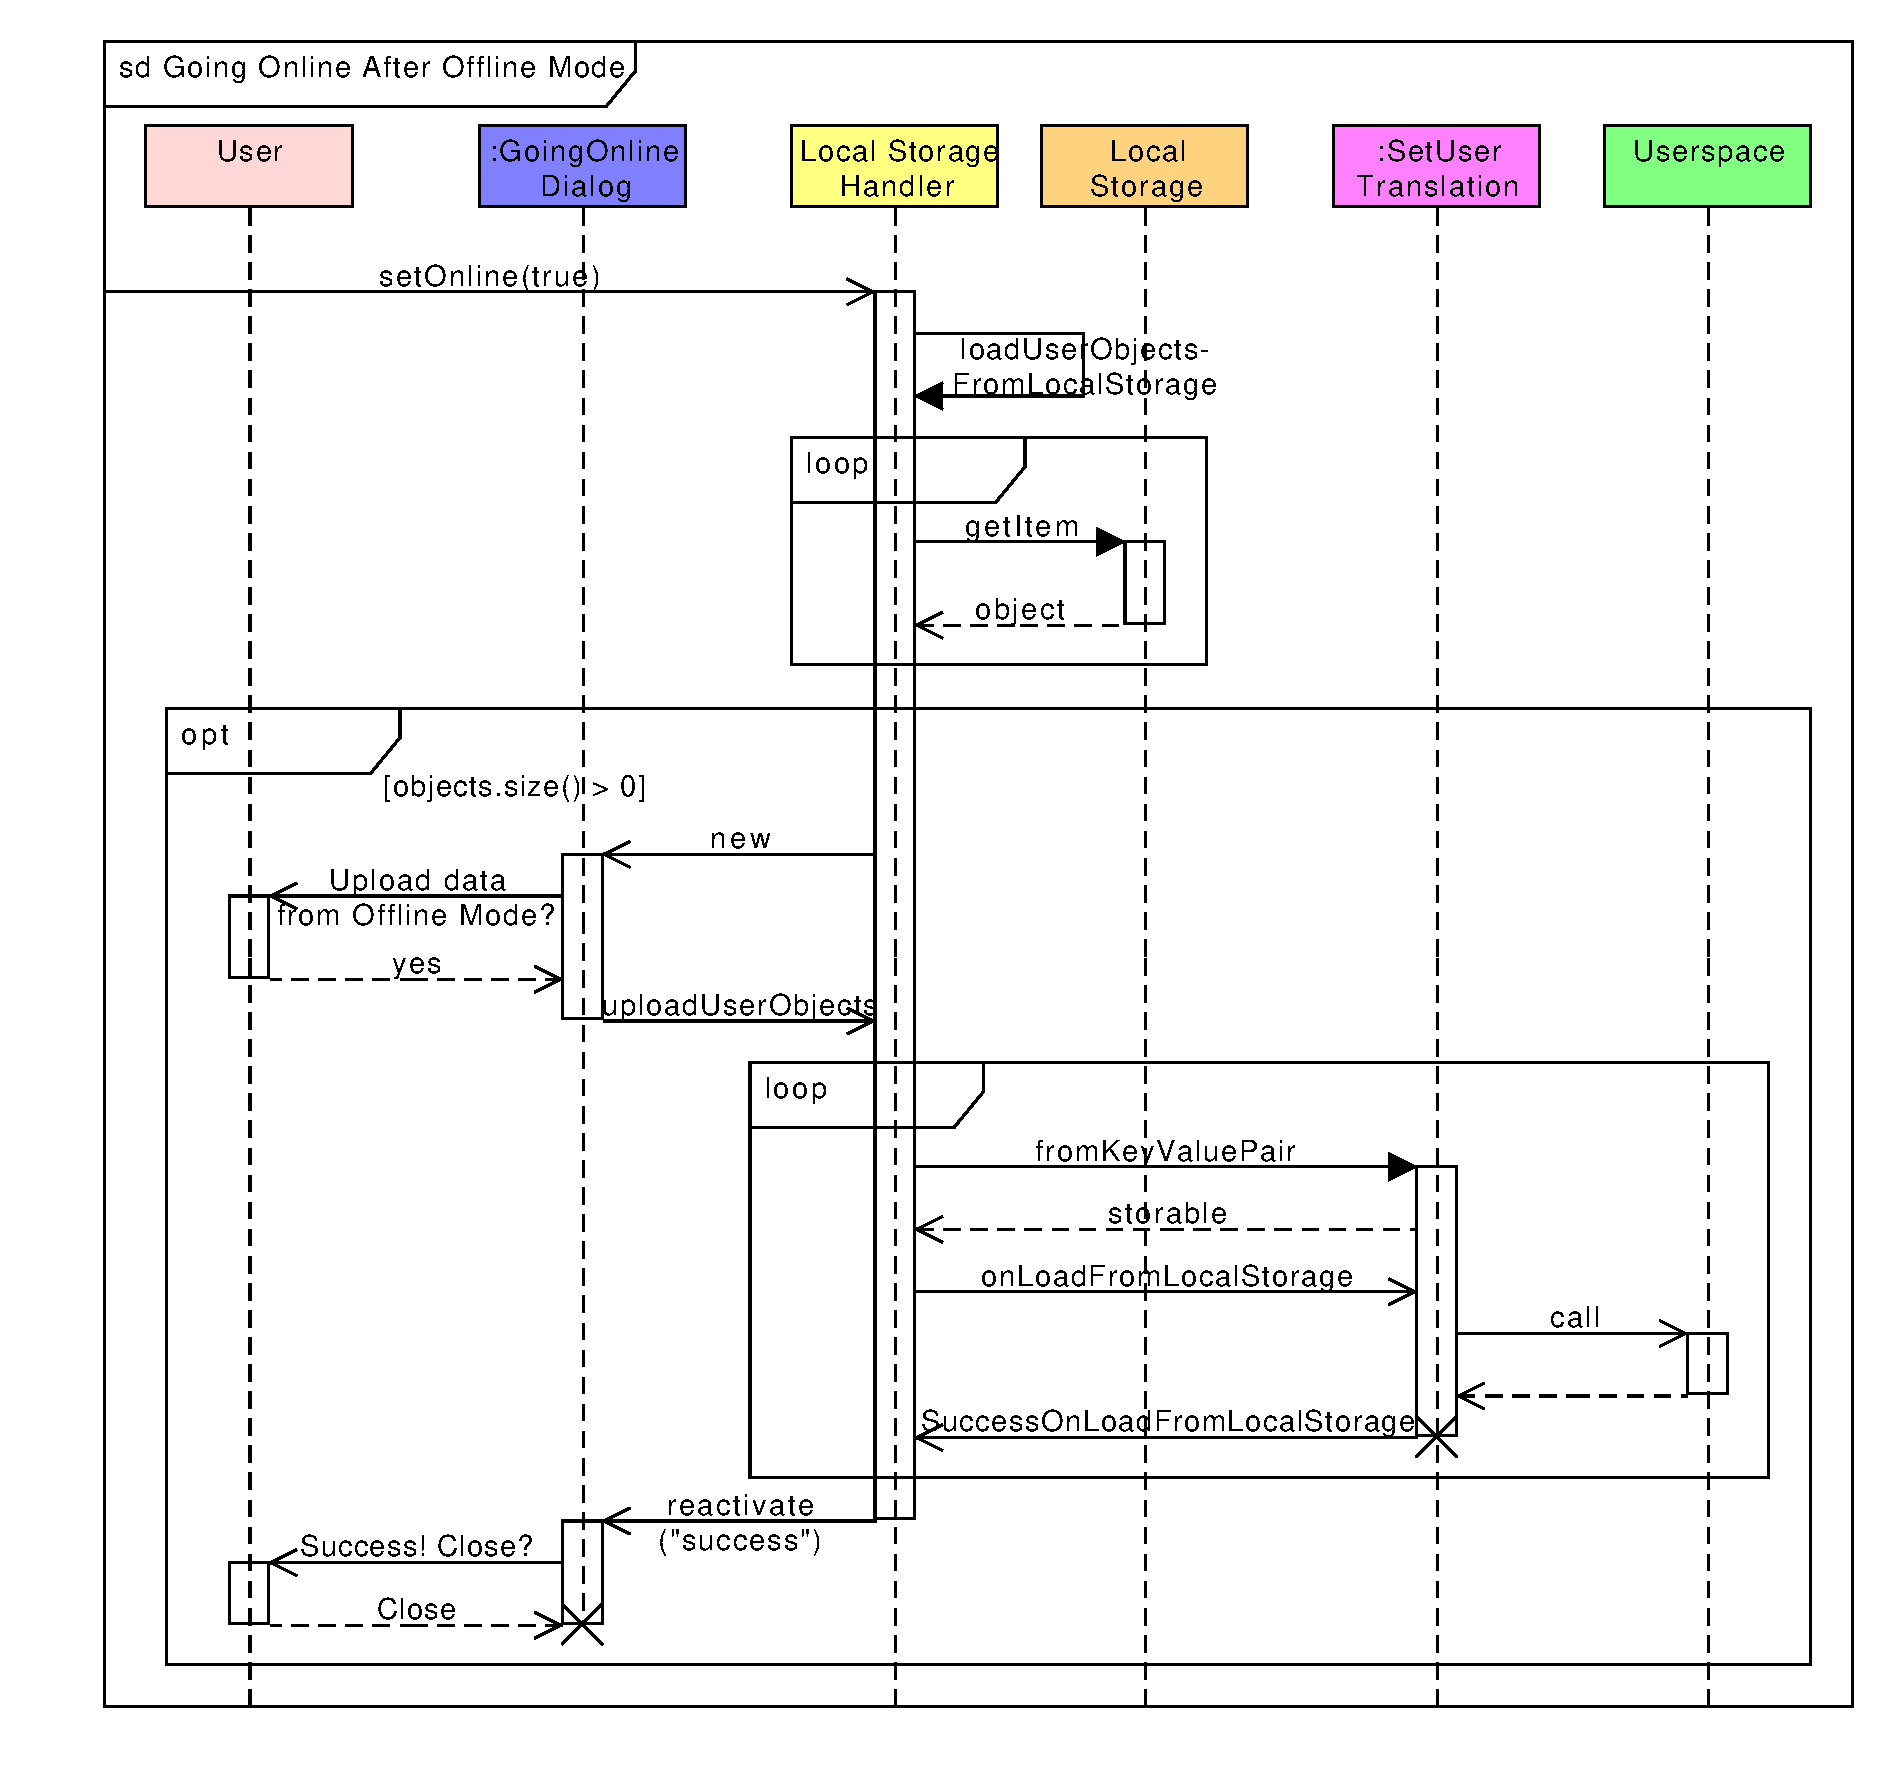
\includegraphics[scale=0.55]{figures/offline_mode_2.pdf}
\end{center}
\caption{Sequence diagram of the user going online after using Offline Mode.}\label{gui:sd:offline_mode_2}
\end{figure}

Before using the Local Storage, it is checked whether it is supported -- if it is not, Offline Mode is not offered to the user and a relevant message is displayed.

When a setUserTranslation call fails with the ``probably offline'' error, it is saved into a queue of failed calls that are to be stored offline if the user agrees (other {\tt setUserTranslation} calls could already have been invoked and will also fail and get enqueued). If the user decides to turn on the Offline Mode, all calls from the queue are stored into Local Storage.

In Offline Mode, the style of the menu is changed and all active components are hidden, because the user should not leave the Translation Workspace while in Offline Mode. Also, going back or forward using the browser controls is disabled: each upcoming page switch is cancelled.

The {\tt SetUserTranslation} calls invoked while in Offline Mode are not sent to server, but they are serialized into a key-value pair and stored in the Local Storage.

Once the user is back online and logs in again, the {\tt LocalStorageHandler} examines the Local Storage. It strips the {\tt userID} part of the key of each object found and compares it to the currently logged in user. If some data belonging to the users are found, they are informed about their count and are suggested to upload the data. If they agree, {\tt LocalStorageHandler} goes through the data, stripping off the ClassID and invoking the corresponding ``{\tt ClassID.fromKeyValuePair()}'' deserialization. Subsequently, the {\tt onLoadFromLocalStorage()} method is invoked on each of the resulting objects -- the {\tt SetUserTranslation} implementation of this method is to invoke the {\tt setUserTranslation call}, i.e.\ to store the translation on the server. When the call returns, {\tt LocalStorageHandler.SuccessOnLoadFromLocalStorage()} or {\tt LocalStorageHandler.FailureOnLoadFromLocalStorage()} is called, as required.

When each of the loaded objects has either succeeded or failed, the user is informed about the result. In case of errors, he can decide to retry loading the failed data or to delete them.

\subsection{SubgestBox}
\label{gui:subgest}

An important class is the {\tt SubgestBox}, or ``SUBtitle sugGESTion BOX'', which provides a textbox-like interface and visualizes the TM results, offering a variety of means of navigation through them. It is based on the IFrame HTML element to support also multi-line and formatted inputs. The TM results are shown as a pop-up suggestion list when the textbox is focused. Another features like auto-scrolling to a certain place of the screen and height auto-adjustment for multi-line inputs were added to improve the user experience. The behaviour and features mentioned requires a custom event handling, this is provided by the SubgestHandler class (common to all the SubgestBoxes within a Translation Workspace).

Because of performance reasons, the SubgestBoxes in the Translation Workspace are not initially all loaded as IFrames (since it would cause a heavy load for the browser to handle), but as simple text-areas instead. The conversion to the ``real'' SubgestBoxes only takes place at the moment of their first focusing. The preliminary text-areas are represented as objects of the FakeSubgestBox class, inner class of the SubgestBox.

\subsection{Playing the Movie Files}

From the beginning, we wanted to be able to show the user the movie file along with translations. However, legal issues, bandwidth issues and disk issues bar us from actually uploading the files to our servers -- so, we tried to implement a browser-based player for the users' movie files. Users should be able to play movies from their disks in the browser, and the translation workspace should be able to communicate with this player via JavaScript.

For this, we have to deal with two problems.

\subsubsection*{Video playback (VLCWidget)}

Playing the movie locally, from disk, is actually the lesser problem. We use the VLC browser plugin for that.

VLC\footnote{\url{http://www.videolan.org/vlc/}, short for VideoLan Client} is a popular open source media player. One of its advantages is that it can handle almost any video format and any popular codec available.

VLC has also a feature called ``browser plug-in''\footnote{For some reason, its name is different across the VLC documentation. Sometimes, the name ``Mozilla plug-in'' is used, sometimes ``Web plug-in'', sometimes ``browser plug-in''.}. The browser plug-in is not a part of the standard VLC installation, but can be installed easily.

This browser plug-in can be used for playing local files in the browser, given that the file address is known. It is possible to rewind forward/backward/stop, all through JavaScript.

There are some slight difficulties in the plug-in, though. One of them is, that it is not possible to jump on an exact time location in the video file. Most video files have so-called seek frames, which can appear more or less often (depending on the setting of the encoder), and the VLC plugin always moves to the closest preceding seek frame. The difference can be quite big (even up to 20 seconds). This bars us from playing exactly the time slot of a given subtitle.

The other difficulty is that sometimes, the plugin just freezes without any warning after a move to a position. We have found out that it is somehow connected to the files played; with the exact same movie files, the exact same positions cause the player to crash, but slightly moved positions are not problematic.

The first issue is solved by not playing just the part with one subtitle, but bigger, 30 seconds ``windows''. The entire movie is split into these 30 second windows, and once the user switches from the subtitle in one window to a subtitle in another window in the {\tt TranslationWorkspace}, the whole new window is played. It is actually better than playing just the time of the subtitle, since the user has more context to translate the movie's sentences.

The second issue is resolved by detecting the crashes and restarting the whole plugin in the case of a crash with slightly moved windows.

The entire player is implemented in \texttt{cz.filmtit.client.widgets.VLCWidget}. Apart from that, the \texttt{VLCWidget} displays the subtitles on the left and on the right of the VLC browser plugin (original subtitles on the left, translated on the right).

We intentionally did not implement very sophisticated controls for the player (since it would make the design too complicated). The functionality of the player is restricted to replaying the whole current window or pausing the playing.

\subsubsection*{Java applet for reading the filename}
The bigger problem is actually \emph{reading the name of the file} before giving it to VLC player plugin.

Modern browsers are generally built to give websites as little access to user's system as possible (and understandably so!). These restrictions include the file paths of uploaded files. Even the recent HTML5 standards that do have access to the file itself cannot read the filename.

The only way we found that would be usable across web browsers and operating systems, was to use a Java applet. Java applets have access to the user's disk and can read the filenames; they have to be signed by a certificate, but that certificate can be self-signed.

This is implemented in \texttt{cz.filmtit.client.widgets.FileLoadWidget}.

The problem with this approach becomes evident -- we are now dependent on two external, non-standard, separate plug-ins for the task of playing video files -- the VLC plugin and the Java plugin. Both have to be installed separately, both often cause issues in various browsers (not only in theory). On the other hand, we achieved the almost impossible task -- playing movie files from user's disk in their browsers. If we therefore warn users that this functionality is experimental and carefully explain the two plugins and their installation, we believe the current implementation is acceptable.



\subsection{Parsing and Segmentation}
We already introduced the parsing in Chapter~\ref{parsing_subs}. As we mentioned there, we are reusing the classes of the {\tt dataimport} module (where we parsed and segmented thousands of files) in the GUI.

More information about the parsing can be found in Chapter~\ref{parsing_subs}.


\subsection{Manipulating with the Documents and Subtitle Items}

The user is provided with the options to change some of the properties of the given document or subtitle item. Within the document listing, they can change the title of a document or the corresponding movie without affecting its contents. Also, in the Translation Workspace, a subtitle item can be edited in more ways than only inside the textboxes. The timing can be changed, which is a useful feature especially when used with the embedded player. The user is also allowed to change the source text, this is used typically when there is an error in the original subtitles, because that could deteriorate the quality of the suggestions for this item.

We do not offer explicit deleting of the chunks; however, the default behavior is that the untranslated chunks are not exported, so not translating a chunk is roughly equivalent to deleting it. We also do not allow to change the source subtitle file (this would actually mean deleting the whole old document and creating a new one, probably only keeping the title -- so we leave this for the user to do himself), although smaller edits can be done directly in Translation Workspace (see above).

Most of the non-textbox editing are accessible via clicking or double-clicking on the corresponding text or number. When there was a doubt about the intuitiveness of such action, a tooltip is provided as a hint for the user.



\section{Logging}
\label{gui:logging}
In User Space and Core, we use \emph{Log4J}, which implements the standard Java Logging interface for logging.

The situation with the GUI is not so easy. GWT provides some default logging tools which work in GWT development mode, but not in production. (As a temporary solution, we used a debugging console in GUI, but it is turned off in the final version.)

The final solution we wrote is what we call ``remote logging''. Important messages are now sent to the server through an RPC, where they are both included into the server log and saved into the database for possible future use (together with the {\tt userID} if possible).

The minimal level of a message to be sent to the server can be set (debug, info, warn, error). We log important GUI events and exceptions with their stack traces in order be able to react on potential bug reports later.

There were some technical difficulties -- mainly catching unexpected exceptions in GWT and umbrella exceptions. An umbrella exception is a GWT exception thrown when multiple exceptions have occurred at once, and it contains all of them. Its message and stack trace are not useful at all because they only cover the creation and throwing of the umbrella exception itself, but do not reveal anything about the inner exceptions.

\section{Typical Usage}

\subsection{Document Creation}

In the most typical case, users (already registered) will open the page with FilmTit and log in. Then, they will go to the {\tt DocumentCreator} page to create a new document. A document corresponds to one movie, or more precisely, to one subtitle file being translated from one language to another. On this page, the users should specify the title of the movie (or series), the direction of the translation (e.g.\ from English to Czech) and provide the actual local file with the source subtitles. They can also set a document title different from the movie title, and set a file path to the corresponding movie video file on his file system.
These information are sent to the User Space and, after refining the movie specification through the {\tt MediaSelector}, the new document is created and the page switches to {\tt TranslationWorkspace}, filled with source subtitles (segmented to chunks) together with their timing on the left side and corresponding empty translation text-boxes on the right side.

See also the corresponding sequence diagram \ref{gui:sd:document_creation}.

\begin{figure}[h]
\begin{center}
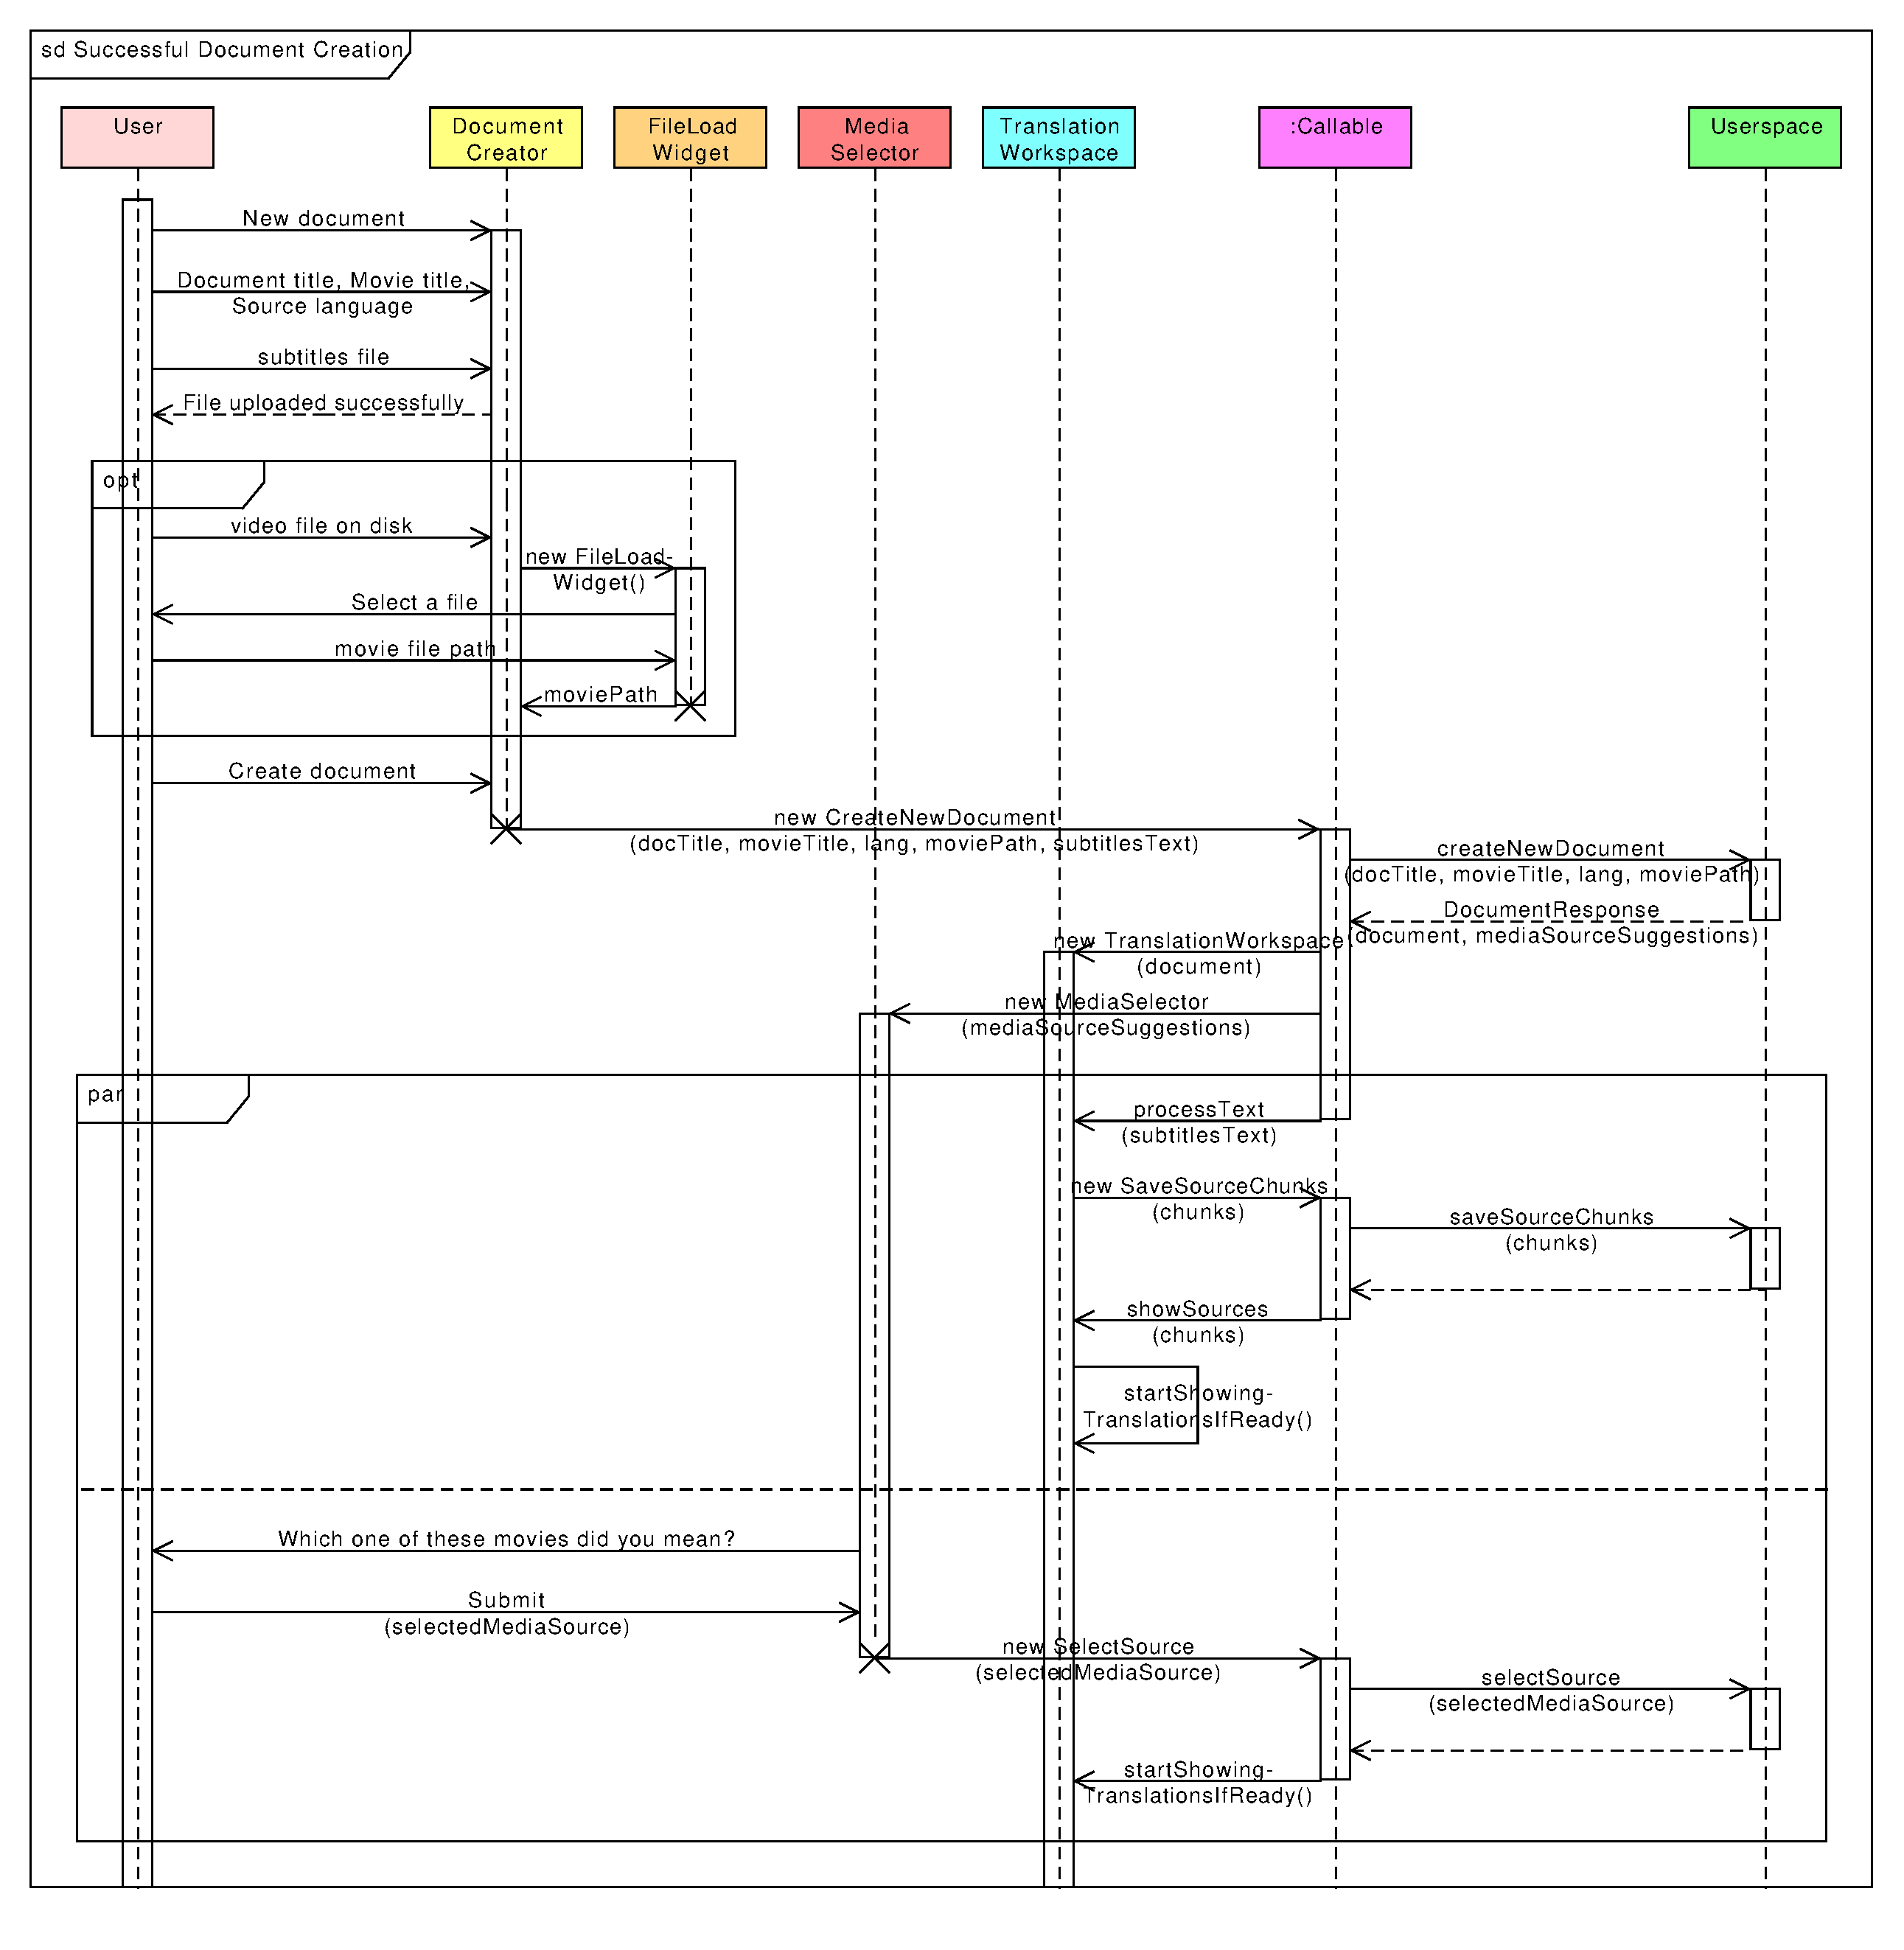
\includegraphics[scale=0.40]{figures/document_creation_sequence_GUI.pdf}
\end{center}
\caption{Sequence diagram of document creation.}\label{gui:sd:document_creation}
\end{figure}

\subsection{Document Translation}
\label{sec:document_translation}

At the same time, the subtitle chunks are sent through the User Space to the Core, where the appropriate translation suggestions are generated for them and sent back. When received in the GUI, each translation result is set to the {\tt SubgestBox} corresponding to its chunk, and can be displayed on activation of the translation text-box as a pop-up, with the suggestions sorted according to their estimated accuracy.
The user can then choose any one of them (or none) and edit it (if necessary) to get the translation of the particular chunk. When the users leave the translation text-box, their translation is sent to the User Space through the {\tt setUserTranslation} call to be saved as the user translation of the chunk.

See also the corresponding sequence diagram \ref{gui:sd:document_translation}.
(Some technical details are ommitted for simplicity.)

\begin{figure}[h]
\begin{center}
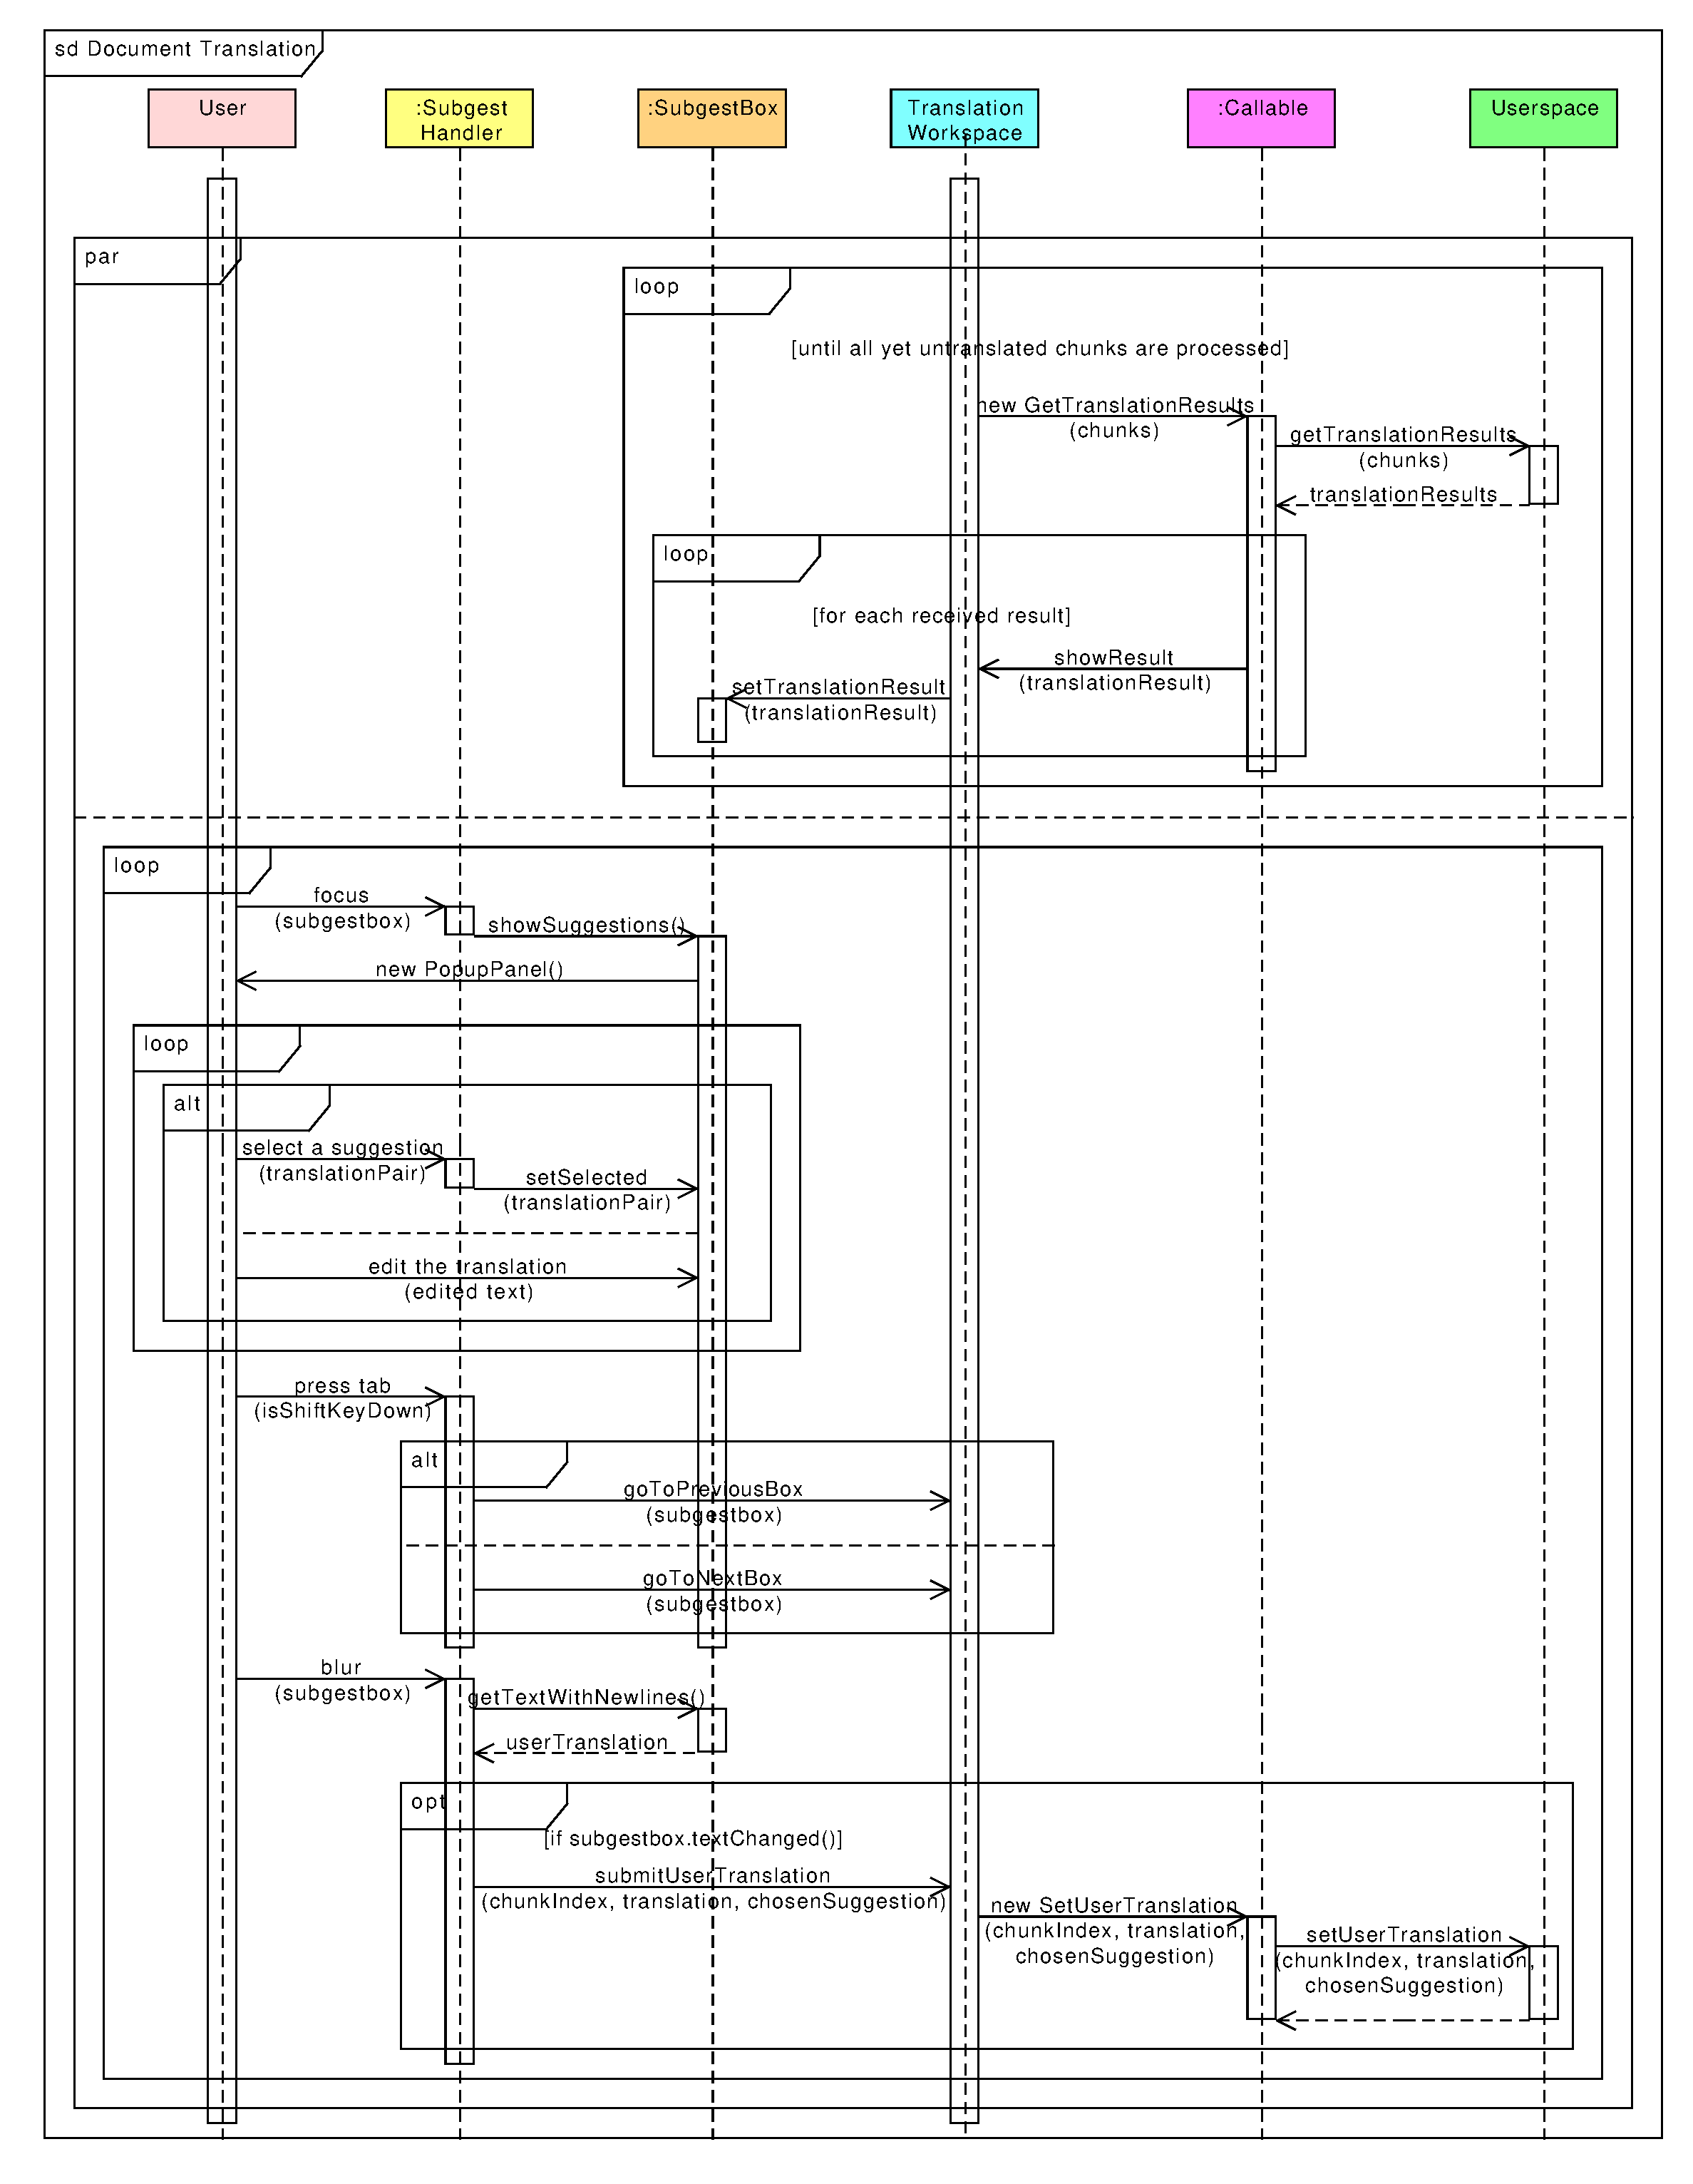
\includegraphics[scale=0.45]{figures/document_translation_sequence.pdf}
\end{center}
\caption{Sequence diagram of document translation.}\label{gui:sd:document_translation}
\end{figure}